\documentclass[11pt]{article}
\usepackage[utf8]{inputenc}
\usepackage[T1]{fontenc}
\usepackage{amsmath}
\usepackage{amssymb}
\usepackage{multicol}
\usepackage{geometry}
\usepackage{tikz}
\usepackage{enumitem}
\usepackage{xcolor}
\usepackage{titlesec}

% Configurações de layout
\geometry{a4paper, left=1cm, right=1cm, top=0.5cm, bottom=1.2cm}
\setlength{\columnseprule}{0.4pt}

% Cores para títulos
\titleformat{\section}{\normalfont\Large\bfseries\color{blue}}{\thesection}{1em}{}
\titleformat{\subsection}{\normalfont\large\bfseries\color{red}}{\thesubsection}{1em}{}

\title{\textcolor{red}{Segundo Trimestre: Matemática
    \\Razão e Proporção}}
\author{Professor: Jefferson}
\date{}

\begin{document}

\maketitle
\vspace{-1cm}

\begin{multicols}{2}

\section*{Introdução}

Razão e proporção são conceitos fundamentais da matemática que permitem comparar grandezas e analisar relações entre valores. Esses conceitos aparecem em situações do cotidiano como receitas, escalas, mapas, consumo, velocidade e tempo.

\section*{Razão}

A razão é a comparação entre duas grandezas por meio de uma divisão.

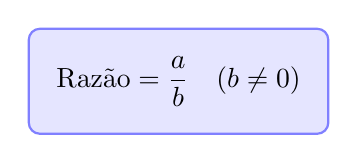
\begin{tikzpicture}
\node[rectangle, fill=blue!10, rounded corners, inner sep=10pt, draw=blue!50, thick] {
$\displaystyle \text{Razão} = \frac{a}{b} \quad (b \neq 0)$
};
\end{tikzpicture}

\textbf{Exemplos:}
\begin{itemize}
\item Razão entre 10 e 5: $\frac{10}{5} = 2$
\item Razão entre meninas e meninos: $12:8$
\item Razão entre distâncias: $3:4$
\end{itemize}

\section*{Proporção}

Proporção é a igualdade entre duas razões.

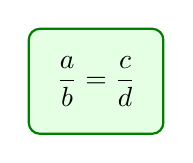
\begin{tikzpicture}
\node[rectangle, fill=green!10, rounded corners, inner sep=10pt, draw=green!50!black, thick] {
$\displaystyle \frac{a}{b} = \frac{c}{d}$
};
\end{tikzpicture}

\textbf{Propriedade fundamental:}
\[
a \cdot d = b \cdot c
\]

\textbf{Exemplo:}
\[
\frac{2}{4} = \frac{3}{6} \Rightarrow 2 \cdot 6 = 4 \cdot 3
\]

\section*{Grandezas Diretamente Proporcionais}

Duas grandezas são diretamente proporcionais quando:
\begin{itemize}
\item Uma aumenta e a outra também aumenta
\item Uma diminui e a outra também diminui
\end{itemize}

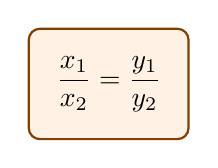
\begin{tikzpicture}
\node[rectangle, fill=orange!10, rounded corners, inner sep=10pt, draw=orange!50!black, thick] {
$\displaystyle \frac{x_1}{x_2} = \frac{y_1}{y_2}$
};
\end{tikzpicture}

\textbf{Exemplos:}
\begin{itemize}
\item Quantidade de produtos e preço total
\item Horas trabalhadas e salário
\item Distância e tempo (velocidade constante)
\end{itemize}

\section*{Grandezas Inversamente Proporcionais}

Duas grandezas são inversamente proporcionais quando:
\begin{itemize}
\item Uma aumenta e a outra diminui
\end{itemize}

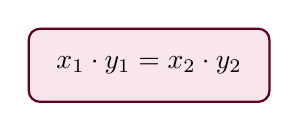
\begin{tikzpicture}
\node[rectangle, fill=purple!10, rounded corners, inner sep=10pt, draw=purple!50!black, thick] {
$\displaystyle x_1 \cdot y_1 = x_2 \cdot y_2$
};
\end{tikzpicture}

\textbf{Exemplos:}
\begin{itemize}
\item Número de trabalhadores e tempo de serviço
\item Velocidade e tempo para percorrer uma distância fixa
\item Quantidade de torneiras e tempo para encher um tanque
\end{itemize}

\section*{Exercícios Básicos}

\begin{enumerate}[leftmargin=*]

\item Calcule a razão:
\begin{enumerate}[label=\alph*)]
\item Entre 12 e 4
\item Entre 15 e 5
\item Entre 8 e 10
\end{enumerate}

\item Verifique se formam uma proporção:
\begin{enumerate}[label=\alph*)]
\item $\frac{3}{5}$ e $\frac{6}{10}$
\item $\frac{4}{7}$ e $\frac{8}{15}$
\item $\frac{9}{12}$ e $\frac{3}{4}$
\end{enumerate}

\item Complete o valor desconhecido:
\begin{enumerate}[label=\alph*)]
\item $\frac{2}{5} = \frac{x}{20}$
\item $\frac{6}{8} = \frac{3}{x}$
\item $\frac{x}{10} = \frac{4}{5}$
\end{enumerate}

\item Identifique se as grandezas são diretamente ou inversamente proporcionais:
\begin{enumerate}[label=\alph*)]
\item Número de pessoas e quantidade de comida
\item Velocidade e tempo de viagem
\item Quantidade de cadernos e preço total
\end{enumerate}

\item Resolva:
\begin{enumerate}[label=\alph*)]
\item Se 5 kg de arroz custam R\$ 25, quanto custam 8 kg?
\item Um carro percorre 120 km em 2 horas. Quantos km percorre em 5 horas?
\end{enumerate}

\section*{Exercícios Contextualizados}

\begin{enumerate}[leftmargin=*, start=6]

\item Uma equipe com 4 operários realiza um trabalho em 12 dias.
\begin{enumerate}[label=\alph*)]
\item Quantos dias seriam necessários com 6 operários?
\end{enumerate}

\item Uma torneira enche um tanque em 10 horas.
\begin{enumerate}[label=\alph*)]
\item Quanto tempo levarão 2 torneiras iguais?
\end{enumerate}

\item Em uma receita, 2 xícaras de farinha rendem 12 biscoitos.
\begin{enumerate}[label=\alph*)]
\item Quantos biscoitos serão feitos com 5 xícaras?
\end{enumerate}

\item Um mapa tem escala 1:100000.
\begin{enumerate}[label=\alph*)]
\item Qual a distância real correspondente a 5 cm no mapa?
\end{enumerate}

\section*{Dicas Importantes}

\begin{itemize}
\item Leia o problema com atenção antes de montar a proporção
\item Identifique se as grandezas são diretas ou inversas
\item Em proporções diretas: iguale as razões
\item Em proporções inversas: iguale os produtos
\item Use regra de três com cuidado
\end{itemize}

\section*{Aplicações Práticas}

\begin{itemize}
\item Cálculo de preços e descontos
\item Ajustes de receitas culinárias
\item Planejamento de tempo e produção
\item Leitura de mapas e escalas
\item Consumo de combustível
\end{itemize}

\end{multicols}

\end{document}

